\documentclass[11pt]{article}

\usepackage[
  a4paper,
  left=20mm,
  right=20mm,
  top=18mm,
  bottom=20mm
]{geometry}
\usepackage{amsmath}
\usepackage{amssymb}
\usepackage{booktabs}
\usepackage{array}
\usepackage{float}
\usepackage{cite}
\usepackage[hidelinks]{hyperref}
\usepackage{graphicx}
\usepackage{siunitx}
\usepackage{etoolbox}
\usepackage{microtype}
\usepackage{placeins}

\newlength{\HFvalidationcolwidth}


\setlength{\parindent}{0pt}
\setlength{\parskip}{4pt plus 1pt minus 1pt}

% Keep figures close to the discussion without forcing premature page breaks.
\setlength{\textfloatsep}{12pt plus 2pt minus 3pt}
\setlength{\floatsep}{10pt plus 2pt minus 2pt}
\setlength{\intextsep}{10pt plus 2pt minus 2pt}
\renewcommand{\topfraction}{0.90}
\renewcommand{\bottomfraction}{0.80}
\renewcommand{\textfraction}{0.08}
\renewcommand{\floatpagefraction}{0.80}
\setcounter{topnumber}{4}
\setcounter{bottomnumber}{2}
\setcounter{totalnumber}{5}

% The bibliography is long; a compact setting avoids a sparsely filled last page.
\AtBeginEnvironment{thebibliography}{%
  \footnotesize
  \setlength{\itemsep}{0pt}%
  \setlength{\parsep}{0pt}%
}

\title{\vspace{-1.2cm}Brief summary of the present $^{273}$Ds and $^{269}$Hs analysis}
\author{Z. R. Sun}
\date{}

\begin{document}
\maketitle

\section*{Purpose}

This note summarizes the current experimental evidence and tentative structural interpretation of two decay chains assigned to $^{273}$Ds, observed in the $^{238}$U($^{40}$Ar,$5n$)$^{273}$Ds reaction at the SHANS-2 separator. The manuscript is still under preparation, and the state assignments discussed below should be regarded as working hypotheses rather than final level assignments.

The main point on which we would appreciate advice is whether the lower-energy, longer-lived $^{273}$Ds decay observed in the present work should be connected with the corresponding long-lived event reported in the DGFRS-2 experiment, or whether the two events should be kept separate at the present stage. This choice affects the estimated hindrance factor and the possible Nilsson-configuration assignment.

\section*{Experimental results}

The experiment was performed at SHANS-2 using the $^{238}$U($^{40}$Ar,$xn$)$^{278-x}$Ds reaction. At an average excitation energy of about 50 MeV, two complete decay chains assigned to the $5n$ channel were observed.
The event-by-event decay sequences are shown in Fig.~\ref{fig:decay-chain}, and the corresponding decay properties are summarized together with previously reported chains in Table~\ref{tab:decay_chains}.
The subsequent decays in both observed chains proceed through $^{269}$Hs, $^{265}$Sg, and terminal spontaneous fission of $^{261}$Rf, and are consistent with previously reported decay properties of these nuclides\cite{habaProduction265Sg2012}.

\begin{figure}[!htbp]
	\centering 
	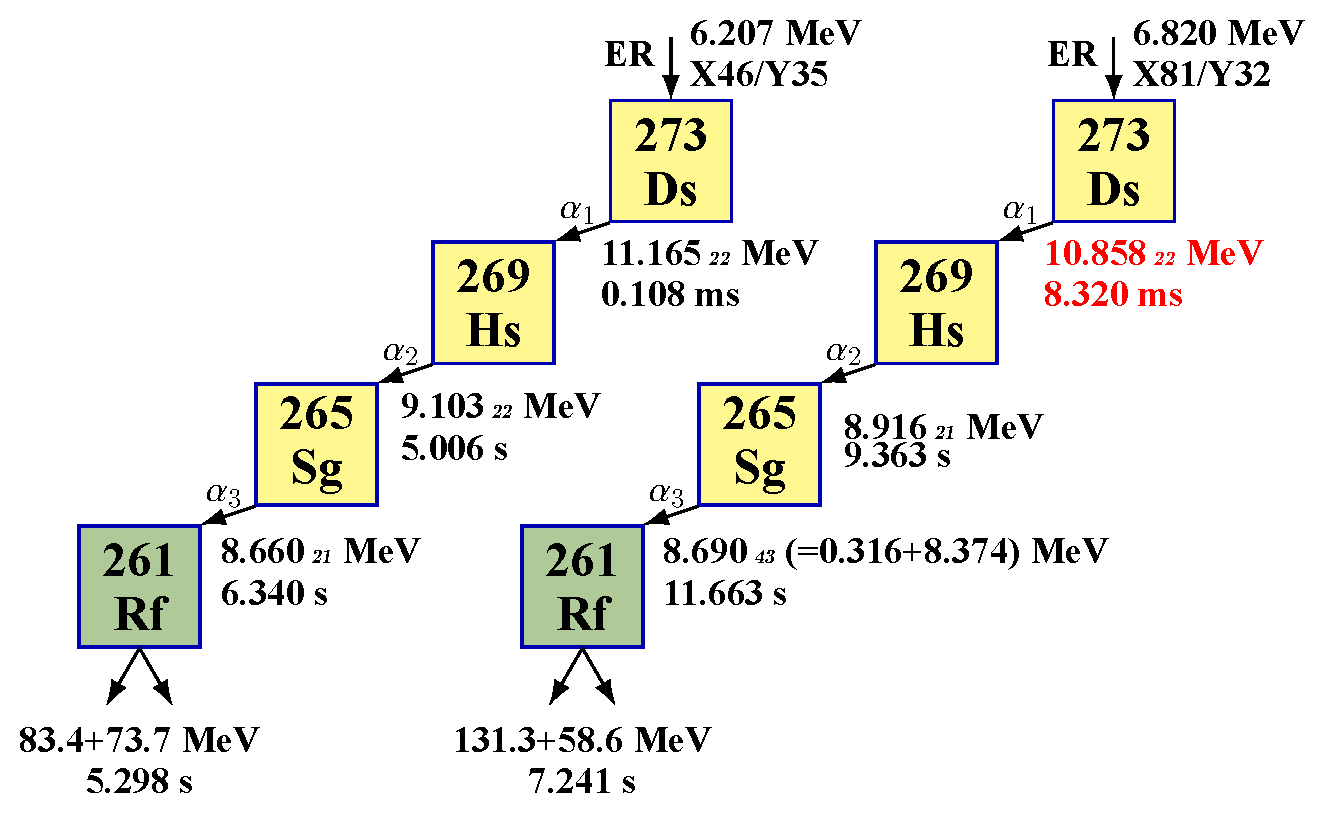
\includegraphics[width=0.74\textwidth]{decayChain.pdf}	
	\caption{Two decay chains assigned to $^{273}$Ds observed in the $^{238}$U($^{40}$Ar, $5n$)$^{273}$Ds reaction. For each chain, the energy of the evaporation residue (ER) event and its $X/Y$ position on the detector are given at the top, followed by the energies of the successive $\alpha$-decay events and the terminal spontaneous-fission (SF) event, together with the time intervals between adjacent events. Energies in parentheses denote summed signals. Italic values indicate the corresponding energy uncertainties. Red text validated in the present work and the inferred assignments related to the isomeric states.} 
	\label{fig:decay-chain}%
\end{figure}

The first chain starts with a higher-energy and shorter-lived $^{273}$Ds alpha decay, whereas the second chain starts with a lower-energy and longer-lived decay. This two-branch pattern resembles that reported in the DGFRS-2 $^{40}$Ar + $^{238}$U experiment\cite{oganessian2024SynthesisDecayProperties}, but the present chains are complete and therefore provide additional information on the daughter decays.
The marked difference in the lifetimes of $^{273}$Ds suggests that the two decay chains originate from two distinct states in $^{273}$Ds. The fact that only the short-lived $^{273}$Ds state has been observed when populated by the $\alpha$ decay of $^{277}$Cn provides further support for the existence of two different states,as shown in Table~\ref{tab:decay_chains}.
\FloatBarrier
\section*{Relation to the DGFRS-2 result}

The long-lived $^{273}$Ds alpha decay in the present work has
\[
E_{\alpha}=10.858(22)\ \mathrm{MeV}, \qquad \Delta t=8.320\ \mathrm{ms}.
\]
The corresponding long-lived event reported in the DGFRS-2 experiment \cite{oganessian2024SynthesisDecayProperties} has
\[
E_{\alpha}=10.929(22)\ \mathrm{MeV}, \qquad \Delta t=41.703\ \mathrm{ms}.
\]
The energy difference is about 71 keV, which is larger than three times the present experimental energy uncertainty. Therefore, although both events belong to the lower-energy, longer-lived branch relative to the known high-energy $^{273}$Ds decay, it is not obvious whether they should be assigned to the same state. The comparison of the available $E_{\alpha}$ and decay-time information in Fig.~\ref{fig:EalphaAndDecaytime} illustrates this ambiguity, and we are considering both possibilities.

\begin{figure}[!htbp]
	\centering 
	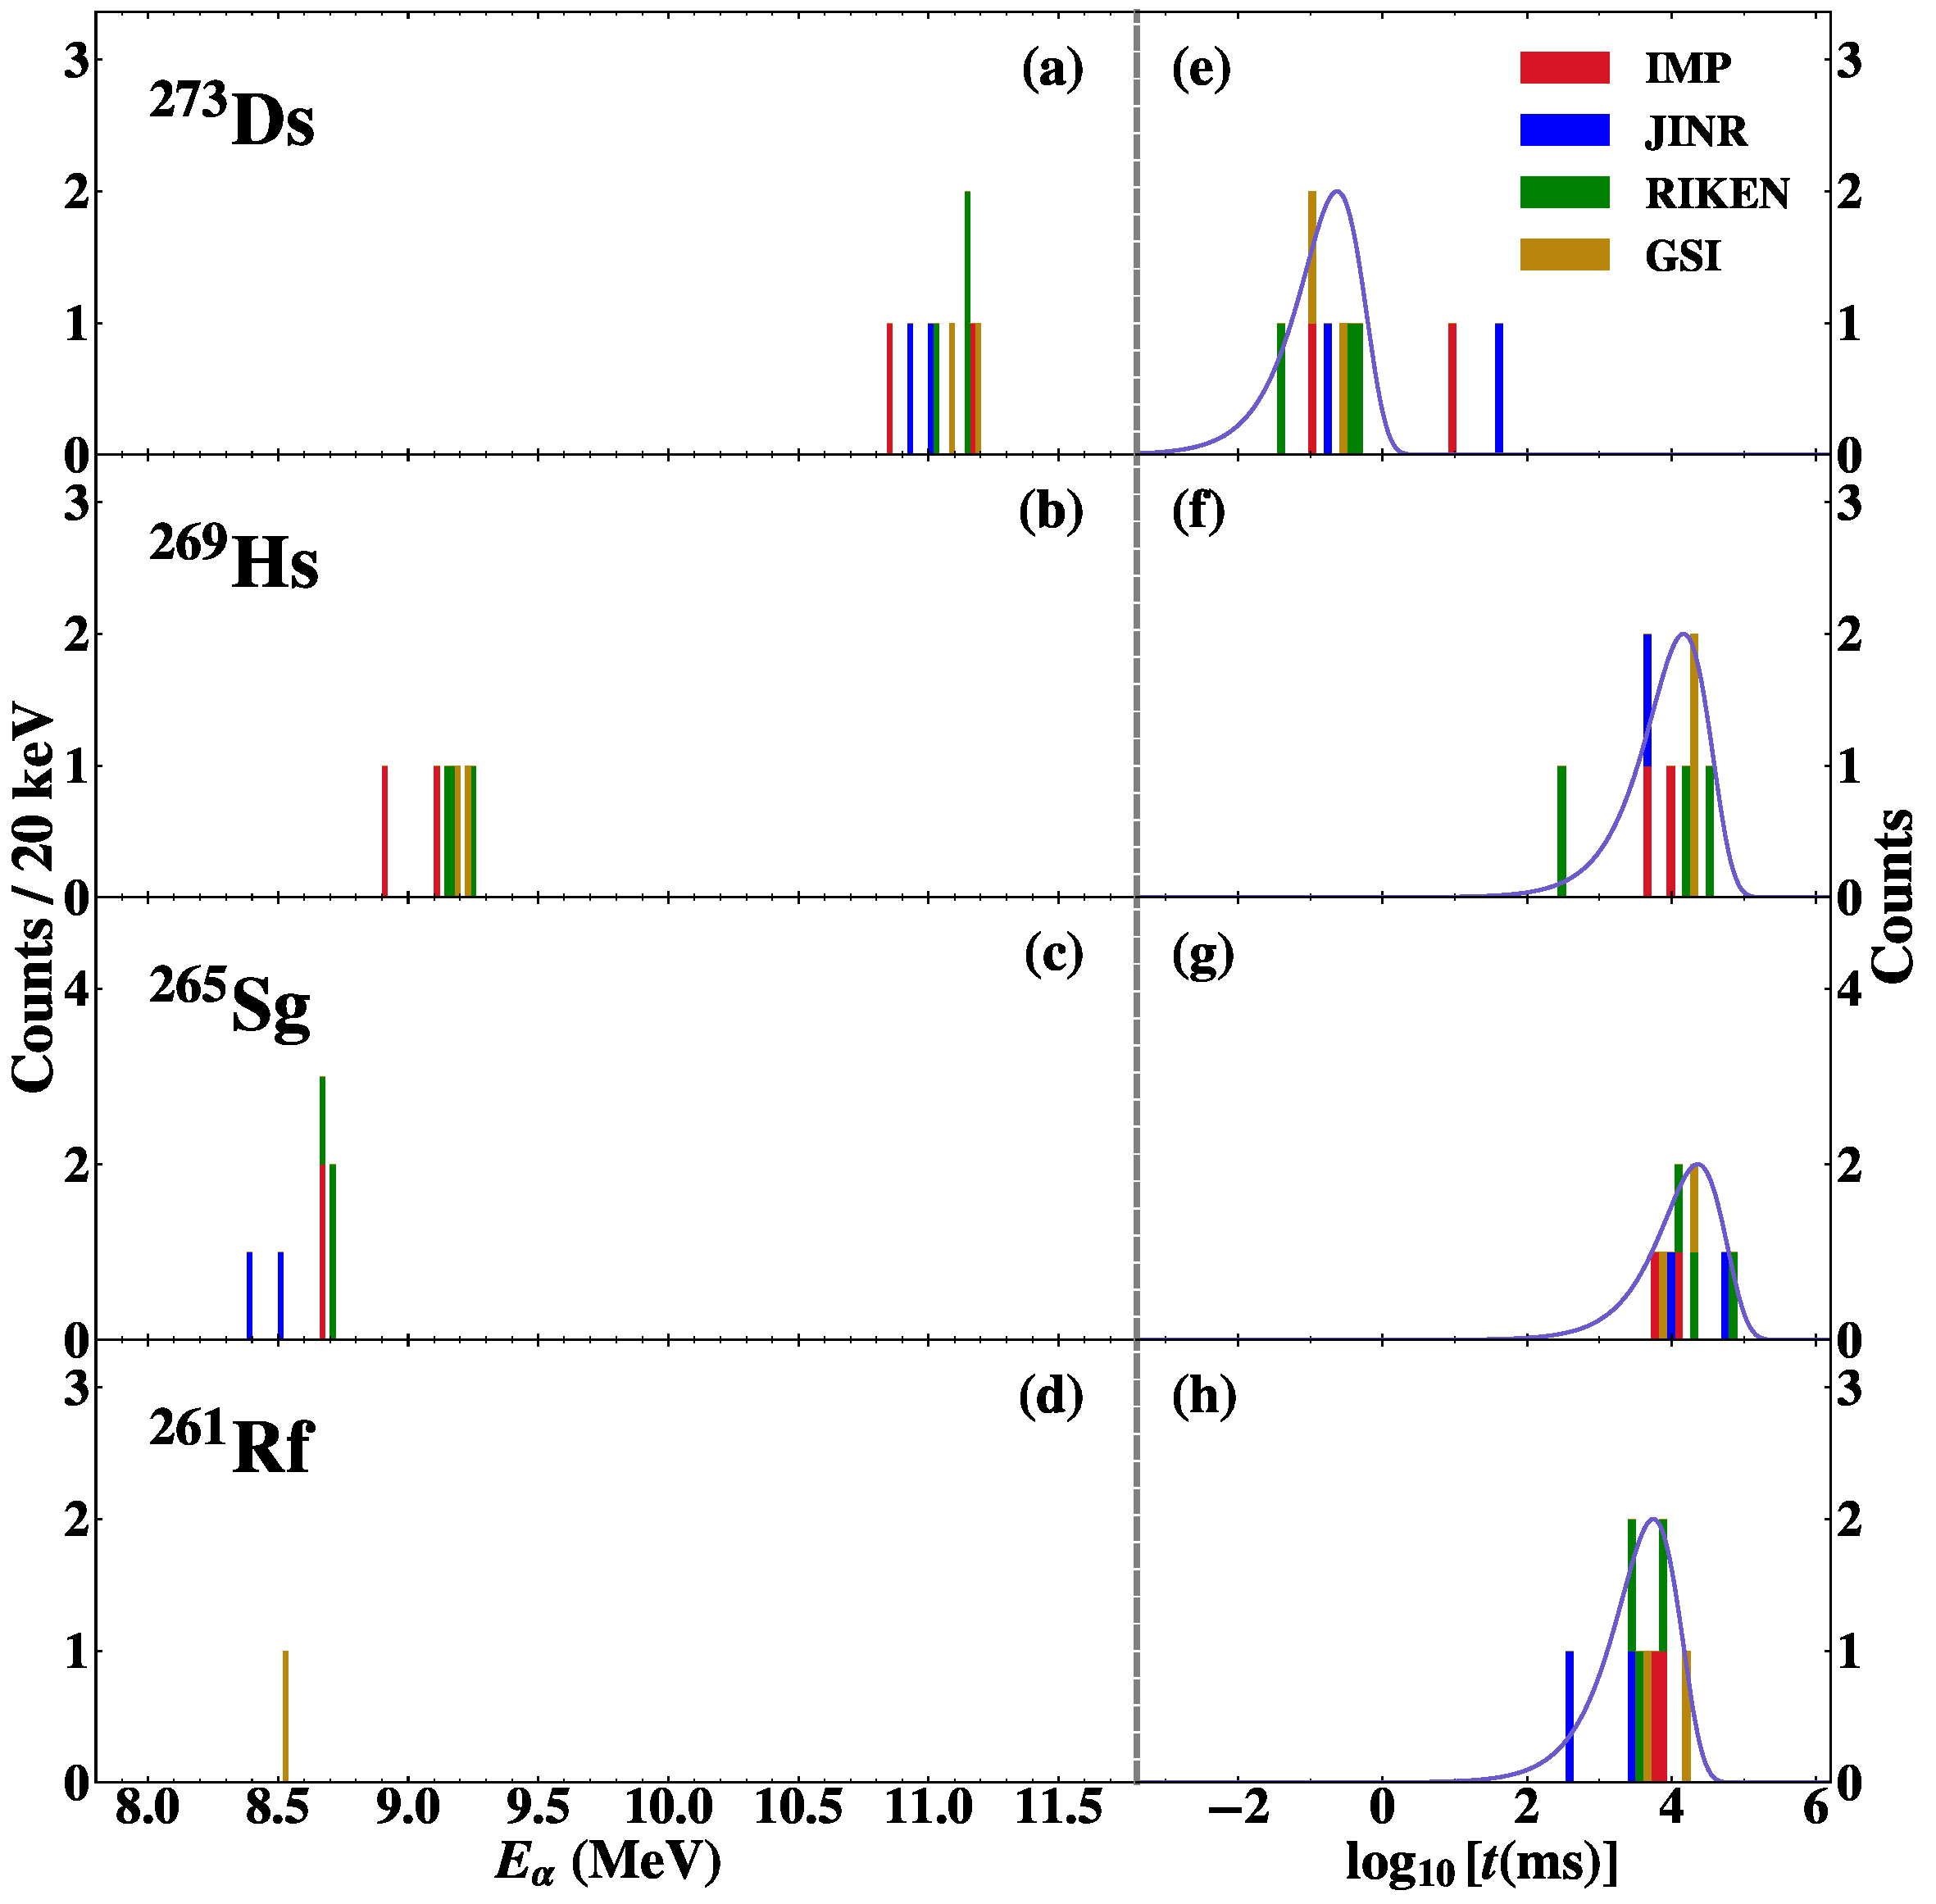
\includegraphics[width=0.60\textwidth]{EalphaAndDecaytime.pdf}	
	\caption{Comparison of the $E_{\alpha}$ and mean life information for decay chains involving $^{273}$Ds. The red, blue, green, and yellow symbols correspond to the IMP, JINR\cite{oganessian2024SynthesisDecayProperties}, RIKEN\cite{sumita2013NewResultProduction,morita2007ExperimentSynthesisIsotope277}, and GSI\cite{hofmann2002NewResultsElements,hofmann1996NewElement112}. The fit curves in the decay-time panels are drawn according to Ref.~\cite{schmidt2000NewTestRandom}.}
	\label{fig:EalphaAndDecaytime}%
\end{figure}

\FloatBarrier
\section*{Possible low-lying state in $^{269}$Hs}

The daughter decay in the long-lived $^{273}$Ds chain has $E_{\alpha}= 8.916\ \mathrm{MeV}$,
which is lower than the higher-energy $^{269}$Hs alpha group near 9.0--9.3 MeV. In the present analysis, the lower-energy $^{269}$Hs group is preferentially associated with the lower-energy, longer-lived $^{273}$Ds branch, whereas the higher-energy $^{269}$Hs group is mainly associated with the higher-energy, shorter-lived $^{273}$Ds branch. No clear cross feeding has been observed within the available statistics.

\begin{table*}[htbp]
\centering
\caption{Decay properties of the observed chains assigned to
$^{277}$Cn, $^{273}$Ds, $^{269}$Hs, $^{265}$Sg, and $^{261}$Rf.
The decay times of individual events are listed.}
\label{tab:decay_chains}
\resizebox{\textwidth}{!}{%
\begin{tabular}{cc
                cc
                cc
                cc
                cc
                cc}
\toprule
\multicolumn{2}{c}{} &
\multicolumn{2}{c}{$^{277}$Cn} &
\multicolumn{2}{c}{$^{273}$Ds} &
\multicolumn{2}{c}{$^{269}$Hs} &
\multicolumn{2}{c}{$^{265}$Sg} &
\multicolumn{2}{c}{$^{261}$Rf}
\\
\cmidrule(lr){3-4}
\cmidrule(lr){5-6}
\cmidrule(lr){7-8}
\cmidrule(lr){9-10}
\cmidrule(lr){11-12}

No. &
Reference &
$E_{\alpha}/ \mathrm{MeV}$ &
$\Delta t$ /$\mathrm{ms}$ &
$E_{\alpha}/ \mathrm{MeV}$ &
$\Delta t$ /$\mathrm{ms}$ &
$E_{\alpha}/ \mathrm{MeV}$ &
$\Delta t$ /$\mathrm{s}$ &
$E_{\alpha}/ \mathrm{MeV}$ &
$\Delta t$ /$\mathrm{s}$ &
$E_{\alpha}/ \mathrm{MeV}$ &
$\Delta t$ /$\mathrm{s}$
\\
\midrule

Ch1 & \cite{hofmann2002NewResultsElements}
& 11.45 & 0.280
& 11.08 & 0.110
& 9.23  & 19.7
& (4.60) & 7.4
& 8.52 & 4.7
\\

Ch2 & \cite{hofmann2002NewResultsElements}
& 11.17 & 1.406
& 11.20 & 0.310
& 9.18  & 22.0
& (0.2) & 18.8
& (SF) & 14.5
\\

Ch3 & \cite{morita2007ExperimentSynthesisIsotope277}
& 11.09 & 1.10
& 11.14 & 0.520
& 9.17  & 14.2
& 8.71  & 23.0
& (SF) & 2.97
\\

Ch4 & \cite{morita2007ExperimentSynthesisIsotope277}
& 11.32 & 1.22
& 11.15 & 0.0399
& 9.25  & 0.270
& 8.70  & 79.0
& (SF) & 8.30
\\

Ch5 & \cite{sumita2013NewResultProduction}
& 11.07 & 0.370
& 11.03 & 0.373
& 9.15  & 36.0
& 8.66  & 13.8
& (SF) & 3.73
\\

Ch6 & \cite{oganessian2024SynthesisDecayProperties}
& -- & --
& 11.017 & 0.184
& -- & --
& 8.397 & 9.0766
& (SF) & 3.0344
\\

Ch7 & \cite{oganessian2024SynthesisDecayProperties}
& -- & --
& 10.929 & 41.703
& (0.342) & 4.0978
& 8.509 & 58.19
& (SF) & 0.3923
\\

\midrule

Ch8 & This work
& -- & --
& 11.165 & 0.108
& 9.103  & 5.006
& 8.660  & 6.340
& (SF) & 5.298
\\

Ch9 & This work
& -- & --
& 10.858 & 8.320
& 8.916  & 9.363
& 8.690  & 11.663
& (SF) & 7.241
\\

\bottomrule
\end{tabular}%
}
\end{table*}

This apparent selectivity in the $\alpha$-decay feeding makes it more plausible that the 8.92–9.00 MeV group corresponds to an additional low-lying or isomeric state in $^{269}$Hs, rather than merely to an unresolved $\alpha$-decay branch from the same state. The compiled $^{269}$Hs $\alpha$-energy distribution in Fig.~\ref{fig:HsData_WithEvents} shows how the present low-energy event compares with the directly produced and daughter-populated $^{269}$Hs data. Owing to the inability of previous radiochemical experiments to determine the ER–$\alpha_1$ correlation time, the present work provides the first direct decay time measurement for this low-energy $\alpha$-decay group in $^{269}$Hs. However, its measured lifetime does not appear to differ significantly from those of the other groups. Given the still limited number of events, the proposed classification of states in $^{269}$Hs should therefore remain tentative.

\begin{figure}[!htbp]
	\centering 
	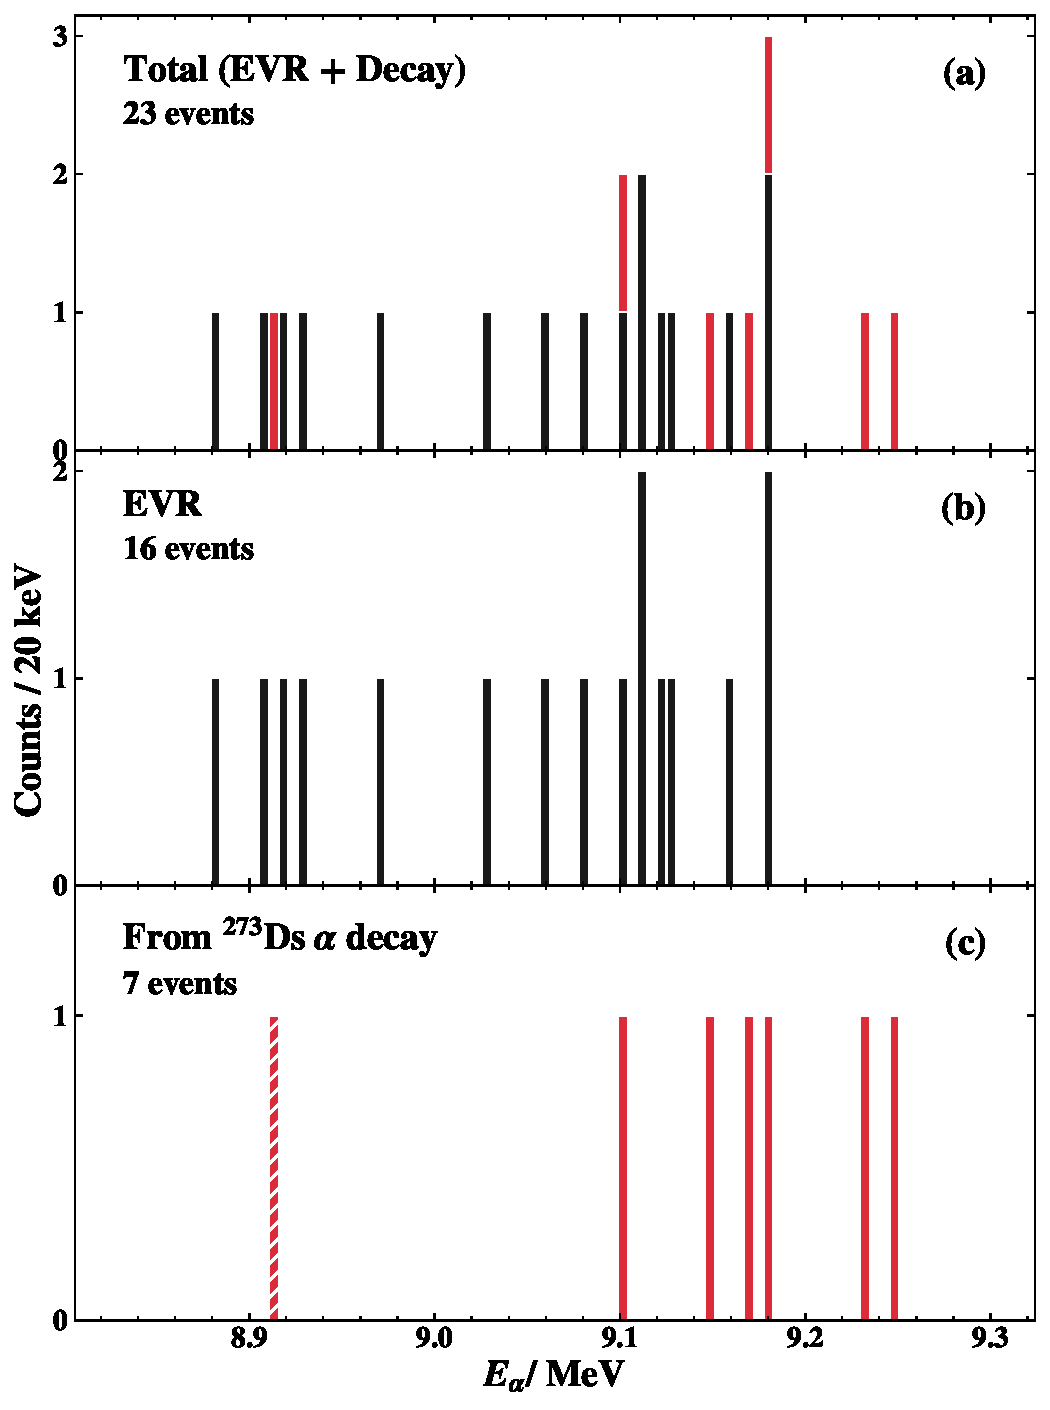
\includegraphics[width=0.52\textwidth]{HsData_WithEvents.pdf}	
	\caption{Energy distributions of $\alpha$ particles assigned to $^{269}$Hs. The upper panel shows all events, the middle panel shows nuclei produced directly as evaporation residues (EVRs)\cite{dvorakDoublyMagicNucleus2006,dvorakObservation3Evaporation2008,turlerNuclearStructureReaction2012,vonzweidorfEvidenceFormationSodium2004}, and the lower panel shows nuclei populated through the $\alpha$ decay of $^{273}$Ds\cite{hofmann2002NewResultsElements,morita2007ExperimentSynthesisIsotope277,sumita2013NewResultProduction}. The hatched bin indicates the event observed in the present work at $E_{\alpha} = 8.916$ MeV.}
	\label{fig:HsData_WithEvents}%
\end{figure}

\FloatBarrier
\section*{Tentative structural interpretation}

\begin{table}[htbp]
\centering
\caption{Decay properties assigned to the long- and short-lived states of $^{273}\mathrm{Ds}$.The half-life of $^{273}\mathrm{Ds}^{a}$ was obtained from a combined analysis of the long-lived decay events observed at JINR and IMP,whereas $^{273}\mathrm{Ds}^{b}$ denotes the short-lived component.The value for $^{273}\mathrm{Ds}^{c}$ was deduced from the single long-lived event observed at IMP only.
The adopted HF calculation procedure was further checked against the
results reported in Table~2 of Ref.~\cite{hessbergerLowLyingIsomers2025};
the comparison is presented in Appendix, Table~\ref{tab:HF_validation}.}
\label{tab:decay_properties}
\begingroup
\renewcommand{\arraystretch}{1.22}
\setlength{\tabcolsep}{7pt}
\begin{tabular*}{0.92\textwidth}{@{\extracolsep{\fill}}lcccc@{}}
\toprule
Nucleus
& \shortstack{$T_{1/2}$\\(\si{\milli\second})}
& \shortstack{$E_{\alpha}$\\(\si{\mega\electronvolt})}
& \shortstack{HF\\ \cite{HFPoenaru,HFE}}
& \shortstack{HF\\ \cite{HFVs}}
\\
\midrule

$^{273}\mathrm{Ds}^{a}$
& $17.34^{+31.55}_{-6.83}$
& $10.89(2)$
& $97^{+183}_{-40}$
& $101^{+192}_{-42}$
\\
\addlinespace[0.25em]

$^{273}\mathrm{Ds}^{b}$
& $0.16^{+0.08}_{-0.05}$
& $11.17(2)$
& $3.8^{+1.9}_{-1.2}$
& $4.2^{+2.1}_{-1.3}$
\\
\addlinespace[0.25em]

$^{273}\mathrm{Ds}^{c}$
& $5.76^{+27.62}_{-2.64}$
& $10.86(2)$
& $27^{+130}_{-13}$
& $28^{+135}_{-13}$
\\

%$^{269}\mathrm{Hs}^{a}$
%& $13^{+10}_{-4}\ \mathrm{s}$
%& $9.20(4)$
%& Ref.~\cite{ref3}

% $^{269}\mathrm{Hs}^{b}$
% & $14.2^{+25.8}_{-5.6}\ \mathrm{s}^{b}$
% & $9.10(2)$
% & this work; Ref.~\cite{ref5}
% \\

% $^{269}\mathrm{Hs}^{c}$
% & $6.49^{+31.09}_{-2.97}\ \mathrm{s}^{b}$
% & $8.92(2)$
% & this work
% \\
\bottomrule
\end{tabular*}
\endgroup
\end{table}

The structural interpretation is based on configuration-constrained potential-energy-surface calculations in the deformation space $(\beta_2,\beta_4,\beta_6)$. 
The nuclear surface is parameterized in terms of spherical harmonics, and the total energy is calculated within the macroscopic--microscopic Strutinsky framework using a realistic phenomenological mean-field Hamiltonian~\cite{brack1972FunnyHillsShellCorrection,xu1998MultiquasiparticlePotentialenergySurfaces,meng2022LandscapeAppreciationSystematic}.
The total energy combines a macroscopic contribution from the standard liquid-drop model~\cite{myersNUCLEARMASSESDEFORMATIONS} with a microscopic contribution comprising the Strutinsky shell correction~\cite{strutinsky1967ShellEffectsNuclear} and the pairing correlation energy. 
The single-particle spectrum is generated from a deformed Woods--Saxon potential using the universal parameter set~\cite{CWIOK1987379}, while pairing correlations are treated with the approximate particle-number-conserving Lipkin--Nogami method~\cite{PRADHAN1973357}, adopting monopole pairing strengths $G$ determined by the average-gap prescription~\cite{MOLLER199220}. 
For each specified one-quasineutron configuration, the unpaired neutron orbital is tracked and blocked at every point on the deformation lattice, thereby treating deformation and pairing consistently for that configuration. 
The calculated Nilsson single-particle levels in
$^{273}\mathrm{Ds}$ and $^{269}\mathrm{Hs}$ as functions of the
deformation parameters $\beta_{2}$, $\beta_{4}$, and $\beta_{6}$
are shown in Figs.~\ref{fig:nilsson_273Ds} and~\ref{fig:nilsson_269Hs},
respectively.
The hindrance factors used to distinguish the long- and short-lived $^{273}$Ds components are listed in Table~\ref{tab:decay_properties}, while the calculated one-quasineutron configurations in $^{273}$Ds and $^{269}$Hs are summarized in Table~\ref{tab:configurations_Ds_Hs}. Their comparison with the observed $\alpha$-decay branches is used to examine possible Nilsson-configuration assignments around the deformed $N=162$ shell closure.
\begin{table}[htbp]
    \centering
    \caption{Calculated one-quasineutron configurations and excitation energies for $^{273}\mathrm{Ds}$ and $^{269}\mathrm{Hs}$.}
    \label{tab:configurations_Ds_Hs}
    \begin{tabular}{l c l c}
        \toprule
        \multicolumn{2}{c}{$^{273}\mathrm{Ds}$} &
        \multicolumn{2}{c}{$^{269}\mathrm{Hs}$} \\
        \multicolumn{2}{c}{$(\beta_2,\beta_4,\beta_6)
        =(0.215,-0.076,-0.006)$} &
        \multicolumn{2}{c}{$(\beta_2,\beta_4,\beta_6)
        =(0.231,-0.062,-0.012)$} \\
        \cmidrule(lr){1-2}
        \cmidrule(lr){3-4}
        Configuration & $E_x$ (MeV) &
        Configuration & $E_x$ (MeV) \\
        \midrule
        $3d_{5/2}\uparrow:\,3/2^{+}[622]$
            & 0.7387
            & $1i_{11/2}\downarrow:\,7/2^{+}[613]$
            & 0.0796 \\
        $1i_{11/2}\downarrow:\,9/2^{+}[604]$
            & 0.6655
            & $1j_{15/2}\downarrow:\,11/2^{-}[725]$
            & 0.0397 \\
        $3d_{5/2}\uparrow:\,5/2^{+}[613]$
            & 0.4730
            & $2g_{7/2}\downarrow:\,1/2^{+}[620]$
            & 0.0292 \\
        $2g_{7/2}\downarrow:\,3/2^{+}[611]$
            & 0.3192
            & $2g_{9/2}\uparrow:\,9/2^{+}[615]$
            & 0.0058 \\
        $1j_{15/2}\downarrow:\,13/2^{-}[716]$
            & 0
            & $3d_{5/2}\uparrow:\,3/2^{+}[622]$
            & 0 \\
        \bottomrule
    \end{tabular}
\end{table}

In this region, $^{273}$Ds can be viewed as containing one neutron above the $N=162$ gap, while $^{269}$Hs contains one neutron hole below it. 

Given the near degeneracy of the relevant one-quasineutron configurations in $^{269}\mathrm{Hs}$, the observed difference in $Q_{\alpha}$ between the two decay chains may primarily reflect the energy separation between the corresponding states in $^{273}\mathrm{Ds}$. 
Two working scenarios are being considered, as illustrated in Fig.~\ref{energylevel}.

\begin{figure}[p]
    \centering
    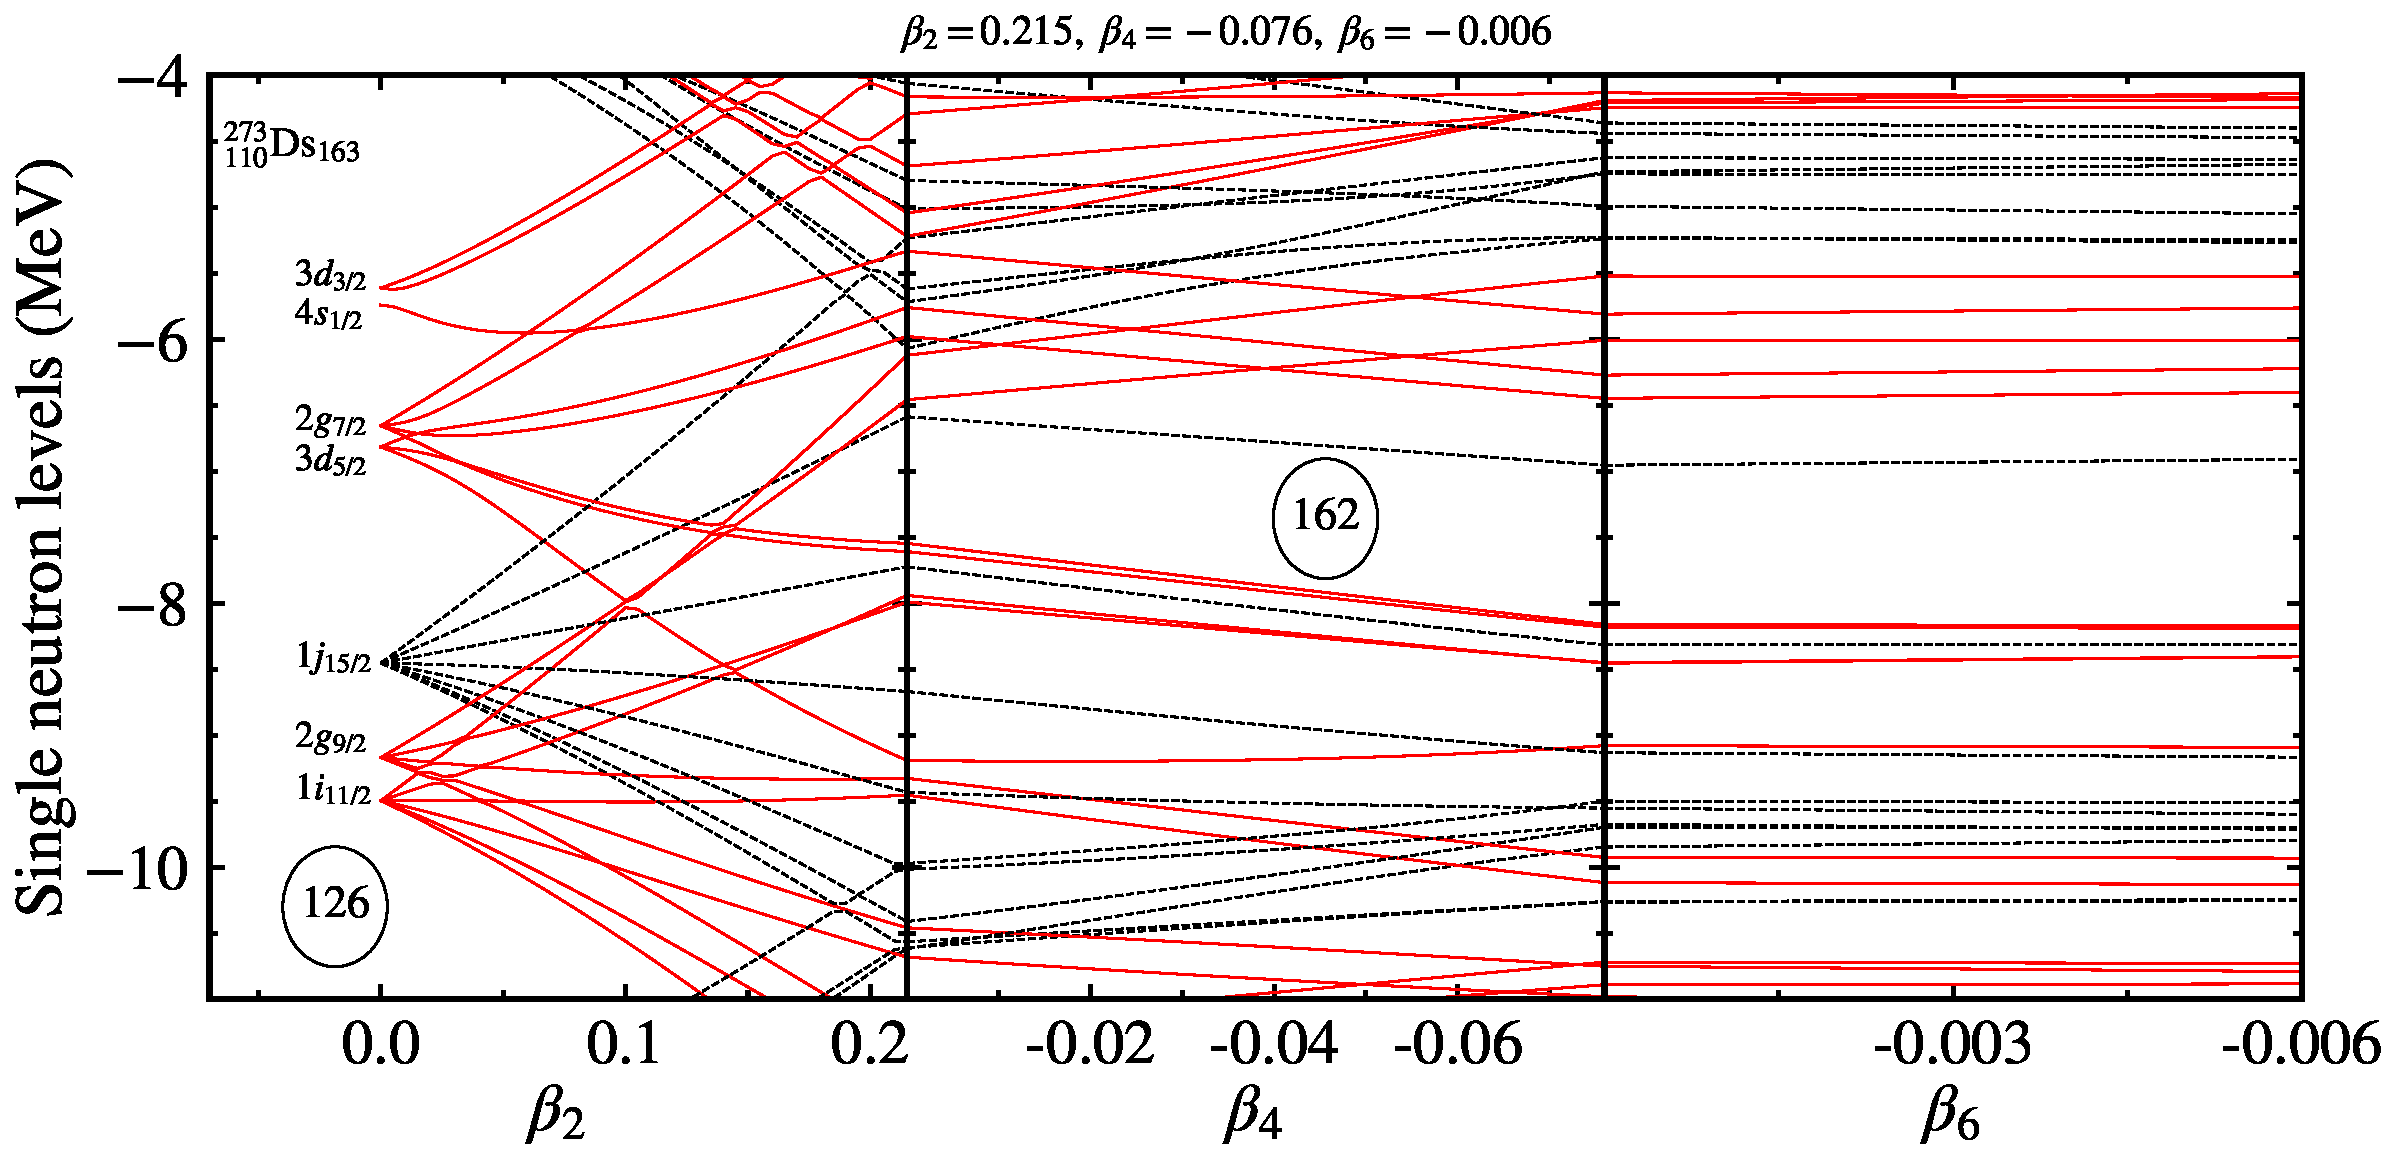
\includegraphics[width=0.76\textwidth]{273Ds_n.pdf}
    \caption{Calculated Nilsson single-particle levels in
    $^{273}\mathrm{Ds}$ as functions of the deformation parameters
    $\beta_{2}$, $\beta_{4}$, and $\beta_{6}$.}
    \label{fig:nilsson_273Ds}

    \vspace{4pt}
    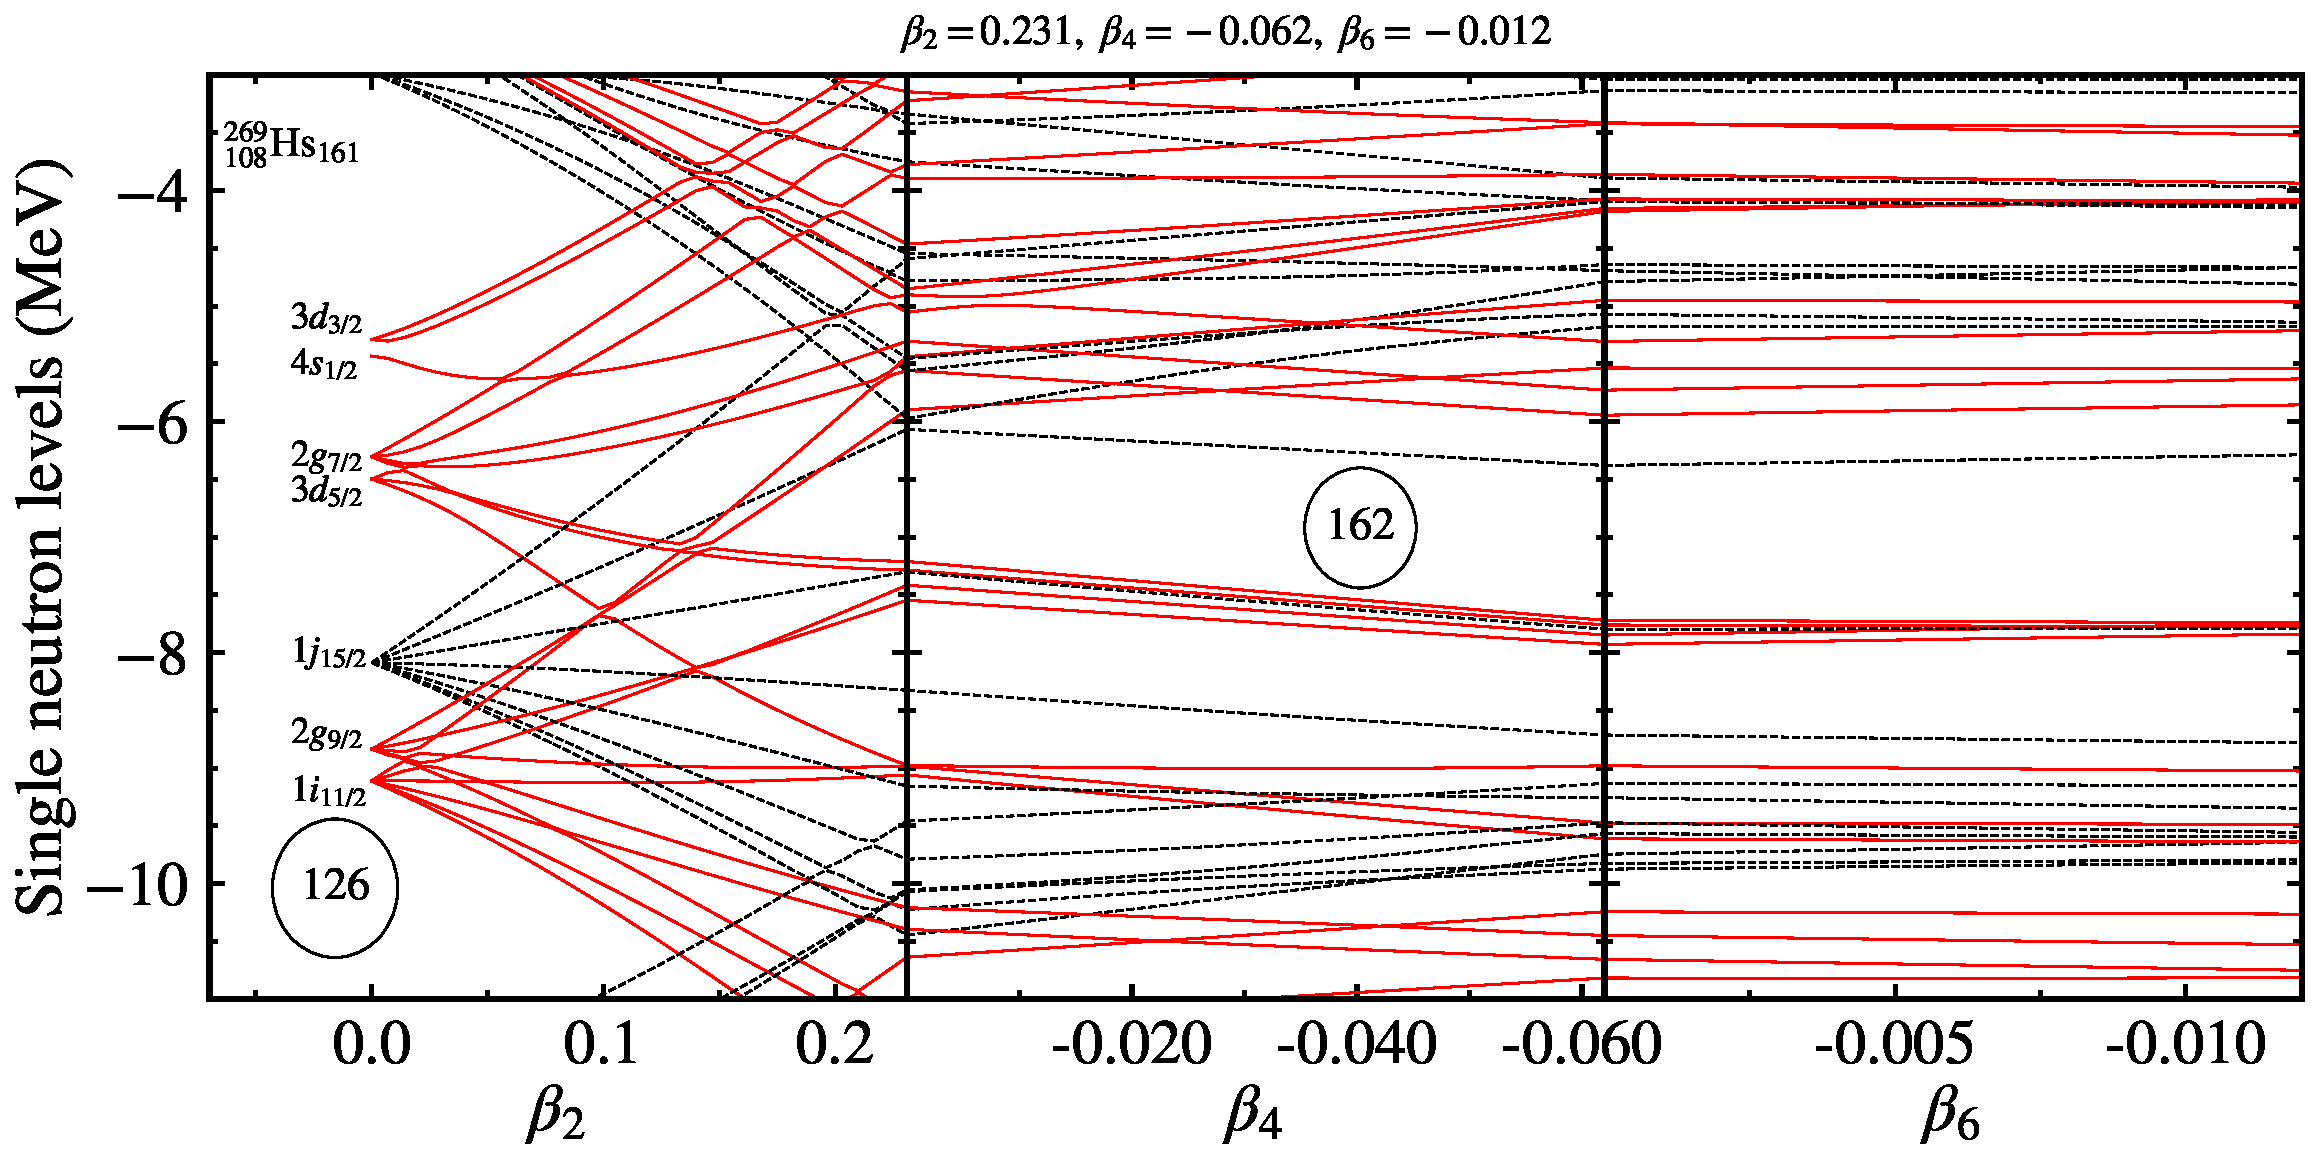
\includegraphics[width=0.76\textwidth]{269Hs_n.pdf}
    \caption{Calculated Nilsson single-particle levels in
    $^{269}\mathrm{Hs}$ as functions of the deformation parameters
    $\beta_{2}$, $\beta_{4}$, and $\beta_{6}$.}
    \label{fig:nilsson_269Hs}

    \vspace{4pt}
    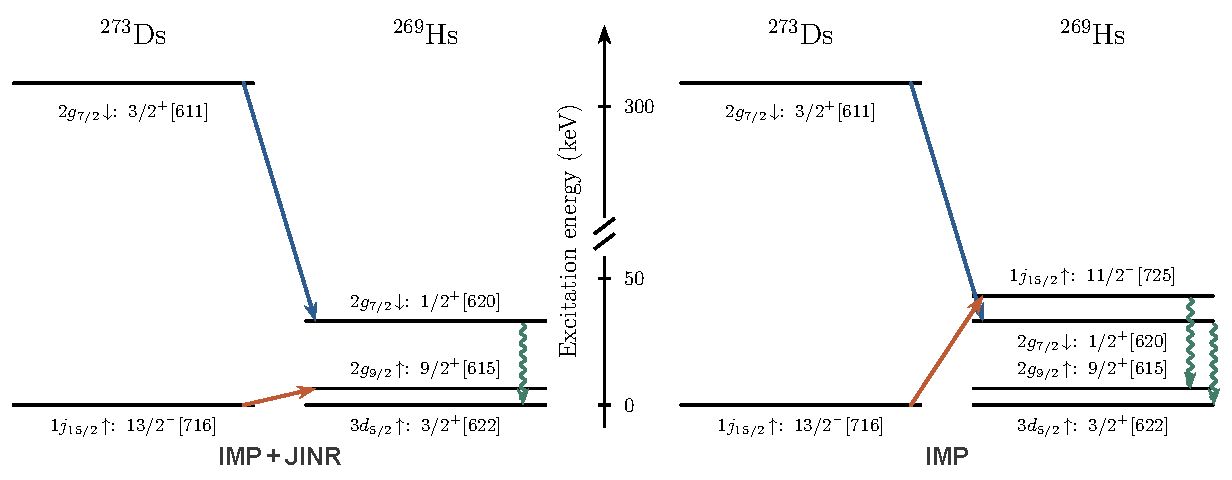
\includegraphics[width=0.76\textwidth]{energylevel.pdf}
    \caption{Comparison of the level assignments for the observed $\alpha$-decay events. In the IMP+JINR interpretation (left), the two long-lived events are assigned to a common state. In the IMP interpretation (right), the IMP event is assigned to a separate state, followed by the indicated $\gamma$ transition to the lower-lying state. The blue arrows denote the short-lived decay transitions, whereas the red arrows denote the long-lived decay transitions. The green wavy arrows indicate the proposed $\gamma$-ray or internal-transition (IT) decays.}
    \label{energylevel}
\end{figure}

At present, neither the hindrance-factor analysis nor the configuration-constrained calculation provides a unique assignment. They are used mainly as consistency checks for possible structural interpretations.

\FloatBarrier
\section*{Systematics and limitations}

\begin{figure}[!htbp]
	\centering
	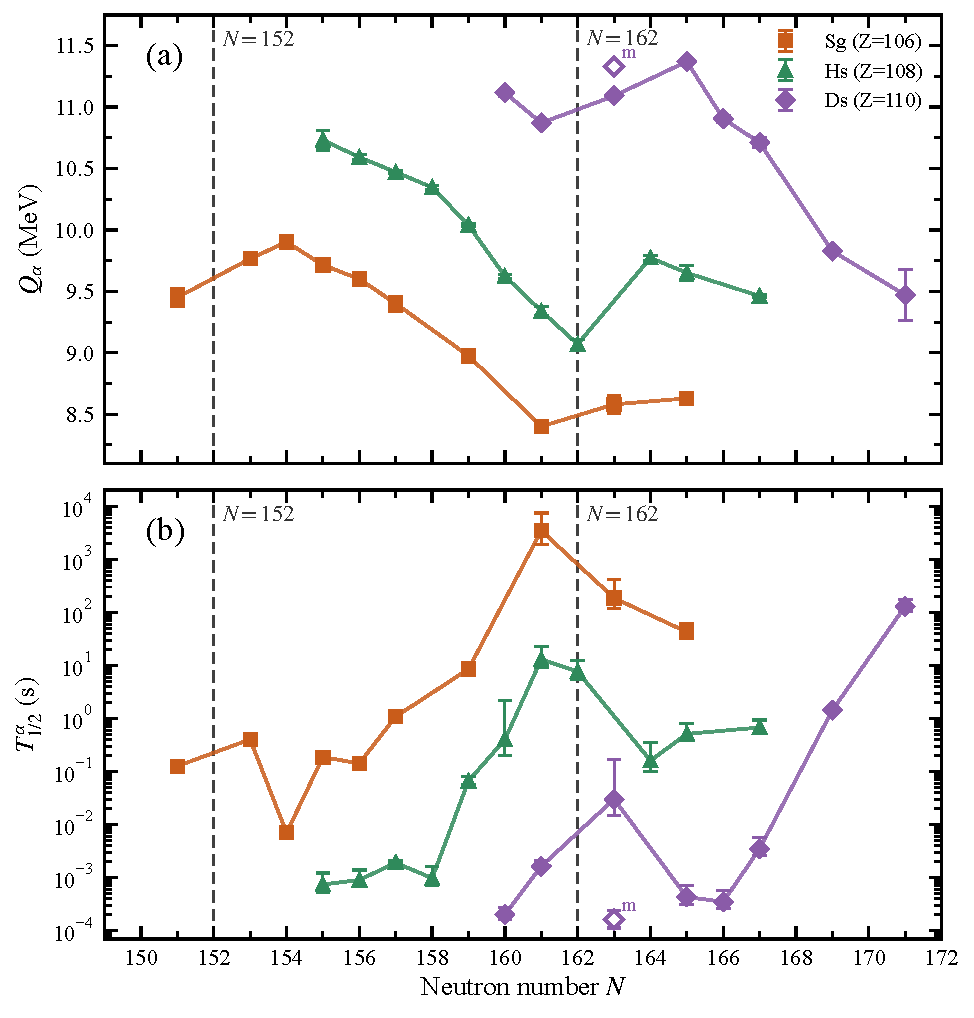
\includegraphics[width=0.70\textwidth]{sys.pdf}
	\caption{Systematics of $Q_{\alpha}$ values and partial $\alpha$-decay half-lives for the Sg, Hs, and Ds isotopic chains. The dashed vertical lines mark $N=152$ and $N=162$. The open diamond labeled m represents $^{273}\mathrm{Ds}^{a}$, whereas the filled diamond connected to the Ds isotopic trend represents $^{273}\mathrm{Ds}^{c}$.}
    \label{fig:System}%
\end{figure}

The isotopic systematics provide a useful broader context for the tentative assignments discussed above. As shown in Fig.~\ref{fig:System}, the $Q_{\alpha}$ values and partial $\alpha$-decay half-lives in the Sg, Hs, and Ds chains do not evolve as a simple monotonic sequence across the deformed $N=162$ region. The local behavior of the Hs and Ds chains is therefore qualitatively compatible with the possibility that different low-lying configurations contribute to the observed decay branches. In particular, the separation between the lower-energy, longer-lived $^{273}$Ds branch and the higher-energy, shorter-lived branch is not inconsistent with a configuration-dependent $\alpha$ decay picture near the deformed shell closure.

This argument should remain modest. The same region is experimentally constrained by Extremely low fusion-evaporation cross sections, so several key nuclei are represented by only one or a few correlated decay chains, and some historical chains are incomplete. As a result, adopted half-lives, partial $\alpha$-decay half-lives, and even branch assignments may be affected by low statistics, unresolved feeding. The systematics in Fig.~\ref{fig:System} should therefore be treated as a consistency check that supports the plausibility of the proposed picture, not as an independent proof of a particular level ordering or Nilsson-configuration assignment. More complete, higher-statistics decay data are needed to fix the ordering in $^{273}$Ds and $^{269}$Hs.

\FloatBarrier
\section*{Open points for discussion}

We would be grateful for comments on the following points.

\begin{enumerate}
\item How reliable are hindrance factors and configuration-constrained calculations for assigning Nilsson configurations in odd-$A$ superheavy nuclei with such limited statistics?
\item The present calculations tend to favor assigning the lower-energy, longer-lived $^{273}$Ds sequence to the ground state and the higher-energy, shorter-lived sequence to a low-lying excited state. Because the available systematics of $Q_{\alpha}$ values and half-lives near $N\approx 162$ are sparse, would such an ordering be reasonable?


\item
Two possible interpretations are currently being considered for the
lower-energy, longer-lived $^{273}$Ds decay.
They differ mainly in whether the 10.858 MeV event observed at IMP and
the 10.929 MeV event observed at JINR should be regarded as the same
$\alpha$-decay transition, different branches from the same parent state,
or unrelated transitions.

\medskip

\textbf{Scenario I: IMP-only interpretation.}

In the most conservative interpretation, the 10.858 MeV event observed
at IMP is treated independently when discussing the microscopic
$\alpha$-decay path. The corresponding half-life gives an empirical
hindrance factor of approximately
\[
\mathrm{HF}\sim 30 .
\]
The preferred long-lived decay path would then be
\[
^{273}\mathrm{Ds}\;
\nu 13/2^{-}[716]
\xrightarrow{\alpha}
^{269}\mathrm{Hs}\;
\nu 11/2^{-}[725]
\xrightarrow{\gamma}
\nu 9/2^{+}[615].
\]
For the $\alpha$ transition,
\[
\Delta K=1,\qquad
\Delta\pi=0,\qquad
l_{\min}=2,
\]
and the initial and final Nilsson orbitals have closely related
$1j_{15/2}$ spherical parentage. This makes the population of the
$\nu 11/2^{-}[725]$ state microscopically natural compared with a
direct transition to the nearby $\nu 9/2^{+}[615]$ state.
The calculated excitation energies of the two states in $^{269}$Hs
differ by only about 34~keV, so there is little energetic penalty for
populating the $\nu 11/2^{-}[725]$ state.

The main difficulty with this interpretation is that the long-lived
transition has $\mathrm{HF}\sim30$, whereas the proposed short-lived
transition,
\[
^{273}\mathrm{Ds}\;
\nu 3/2^{+}[611]
\xrightarrow{\alpha}
^{269}\mathrm{Hs}\;
\nu 1/2^{+}[620]
\xrightarrow{\gamma}
\nu 3/2^{+}[622],
\]
has only
\[
\mathrm{HF}\sim4 .
\]
Both proposed $\alpha$ transitions conserve parity, have
$\Delta K=1$ and $l_{\min}=2$, and approximately preserve their
dominant spherical parentage,$[1j_{15/2}\rightarrow1j_{15/2}$
and $2g_{7/2}\rightarrow2g_{7/2},$
respectively.
Therefore, the difference between $\mathrm{HF}\sim30$ and
$\mathrm{HF}\sim4$ cannot be explained simply by $\Delta K$, parity,
or the minimum transferred angular momentum.
It would therefore have to arise from differences in the detailed
Nilsson-wave-function overlap between the parent and daughter states
and in the corresponding $\alpha$-formation amplitudes.The difference may reflect more detailed differences in the quasiparticle wave functions, 
including those associated with the high-$\Omega$ and low-$\Omega$ character of the orbitals.which are not
evaluated in the present configuration-constrained PES approach.

\medskip

\textbf{Scenario II: IMP+JINR as a common $\alpha$ transition.}

If the 10.858 MeV IMP event and the 10.929 MeV JINR event are assumed
to represent the same long-lived $\alpha$-decay transition, the combined
decay-time analysis gives
\[
T_{1/2}=17.34^{+31.55}_{-6.83}\ {\rm ms},
\]
corresponding to
\[
\mathrm{HF}\sim100 .
\]
Such a large hindrance can be naturally associated with the direct
transition
\[
^{273}\mathrm{Ds}\;
\nu 13/2^{-}[716]
\xrightarrow{\alpha}
^{269}\mathrm{Hs}\;
\nu 9/2^{+}[615],
\]
for which
\[
\Delta K=2,
\qquad
\Delta\pi\neq0,
\qquad
l_{\min}=3,
\]
and the dominant spherical parentage changes approximately from
\[
1j_{15/2}\rightarrow2g_{9/2}.
\]
Thus, if this transition occurs, its large hindrance is qualitatively
easy to understand.

However, this scenario has a different microscopic difficulty.
The calculation predicts the
$\nu 11/2^{-}[725]$ state only about 34~keV above the
$\nu 9/2^{+}[615]$ state in $^{269}$Hs.
The competing transition
\[
\nu 13/2^{-}[716]
\xrightarrow{\alpha}
\nu 11/2^{-}[725]
\]
has
\[
\Delta K=1,\qquad
\Delta\pi=0,\qquad
l_{\min}=2,
\]
and approximately preserves the $1j_{15/2}$ spherical parentage.
On the basis of these gross structural properties, this channel would
normally be expected to be more favorable than the direct transition
to $\nu 9/2^{+}[615]$.

Consequently, the large value
$\mathrm{HF}\sim100$ explains why a
$\nu13/2^{-}[716]\rightarrow\nu9/2^{+}[615]$
transition would be slow, but does not by itself explain why this
strongly hindered branch should be favored over the nearby,
more configuration-preserving
$\nu13/2^{-}[716]\rightarrow\nu11/2^{-}[725]$
transition.Moreover, as discussed in Ref.~\cite{hessbergerLowLyingIsomers2025}, the reliability of the experimental assignment of the JINR event remains open to question.
The present PES calculation does not provide a microscopic
$\alpha$-formation calculation capable of resolving this competition.

\medskip

\end{enumerate}

\section*{Appendix}

\begin{table}[H]
\centering
\caption{
Validation of the hindrance-factor (HF) calculation adopted in the
present work. The HF values calculated are compared with those reported in
Table~2 of Ref.~\cite{hessbergerLowLyingIsomers2025}.
}
\label{tab:HF_validation}
\begingroup
\renewcommand{\arraystretch}{1.22}
\setlength{\tabcolsep}{10pt}
\setlength{\HFvalidationcolwidth}{%
  \dimexpr(0.88\textwidth-10\tabcolsep-\arrayrulewidth)/6\relax}
\begin{tabular}
{@{}*{5}{w{c}{\HFvalidationcolwidth}}|w{c}{\HFvalidationcolwidth}@{}}
\hline
\rule[-0.65em]{0pt}{3.35em}\raisebox{0.5em}[0pt][0pt]{Nucleus}
& \shortstack{$E_{\alpha}$\\(\si{\mega\electronvolt})}
& \shortstack{$T_{1/2}$\\(\si{\milli\second})}
& \shortstack{HF\\ \cite{HFPoenaru,HFE}}
& \shortstack{HF\\ \cite{HFVs}}
& \shortstack{HF\\ \cite{hessbergerLowLyingIsomers2025}}
\\
\hline
$^{271}\mathrm{Ds}$
& $10.44$
& $32$
& $14.24$
& $14.19$
& $14.5$
\\

$^{267}\mathrm{Hs}$
& $9.73$
& $803$
& $21.29$
& $18.05$
& $21.2$
\\

$^{263}\mathrm{Sg}$
& $9.31$
& $4100$
& $33.54$
& $25.44$
& $34.1$
\\
\hline
\end{tabular}
\endgroup
\end{table}


\bibliographystyle{unsrturl}
\begingroup
\let\originalhref\href
\renewcommand{\href}[2]{\originalhref{#1}{\nolinkurl{#1}}}
\bibliography{example}
\endgroup

\end{document}
